%%%%%%%%%%%
% Cristallographie %
%%%%%%%%%%%

\chapter{Notions de base de cristallographie}

\section{Symétrie de translation, réseau et maille}
	On a vu dans le chapitre précédent que la description des cristaux devenait plus compliquée lorsqu'on analysait les cristaux ioniques et les covalents. On a pour ça recours à la cristallographie. 
	\subsection{Définition du réseau}
		\begin{wrapfigure}[4]{l}{2.5cm}
		\vspace{-5mm}
		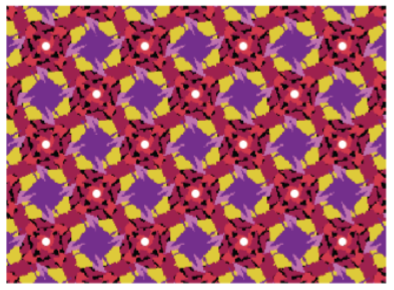
\includegraphics[scale=0.35]{ch4/1}
		\end{wrapfigure}
		Le réseau cristallin d'un monocristal parfait consiste en la répétition infinie, dans les 3 directions de l'espace, d'un même élément appelé \textbf{motif}. La \textbf{position} du motif qui se répète permet de définir les \textbf{noeuds} du réseau. Un réseau n'est pas un arrangement d'atomes mais un arrangement géométrique de points abstraits dans l'espace. 
		
		\begin{wrapfigure}[6]{r}{7cm}
		\vspace{-5mm}
		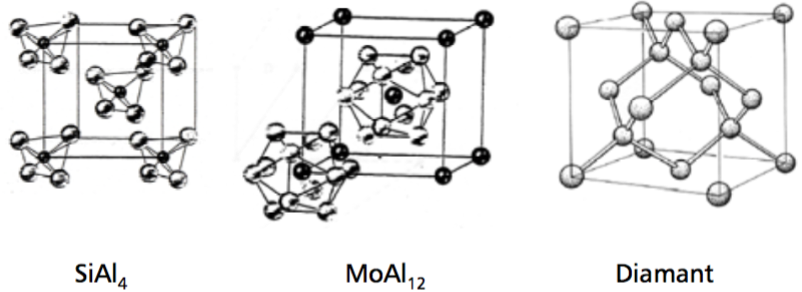
\includegraphics[scale=0.5]{ch4/2}
		\end{wrapfigure}
		Ce concept est illustré ci-contre. Pour les deux premières structures, le motif de base contient respectivement 5 et 13 atomes et sa répartition dans l'espace est selon un cube centré. Le motif peut donc être constitué d'un atome unique ou de plusieurs atomes identiques ou différents dont les positions relatives sont fixées, même pour un solide monoatomique. Pour le diamant, le motif est constitué de deux atomes identiques se disposant selon un cube à faces centrées.   
		
	\subsection{Définition de la translation}
		\begin{wrapfigure}[5]{l}{6.5cm}
		\vspace{-5mm}
		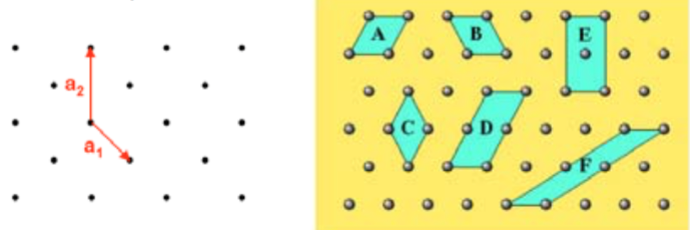
\includegraphics[scale=0.5]{ch4/3}
		\end{wrapfigure}		
		Pour un solide cristallin la symétrie de translation est exigée. Considérons un point quelconque du cristal dont la position est donné par le vecteur $r$. La symétrie existe s'il est possible de choisir trois vecteurs $a_1,a_2, a_3$ tels que l'arrangement local des atomes autour du point $r$ est identique à celui de n'importe quel point $r'$. L'ensemble des $r'$ constitue le réseau. 
		\begin{equation}
			r' = r + n_1a_1 + n_2a_2 + n_3a_3 \qquad n_1,n_2,n_3 \ entiers 
			\label{eq:4.1}
		\end{equation}		 
		On peut voir sur la figure au dessus que les vecteurs $a_i$ peuvent être choisis de différentes manières. Ce sont des \textbf{vecteurs primitifs} si l'ensemble des point $r'$ défini par \autoref{eq:4.1} contient tous les points du cristal équivalent au point $r$. Les deux vecteurs qui engendrent A, B et C sont primitifs mais ceux pour D, E, F non. D'habitude, on prend $a_1$ et $a_2$ perpendiculaires.
		
		
	\subsection{Definition de la maille} 
		A chaque noeud est associé un et un seul motif. Les vecteurs $a_1,a_2,a_3$ définissent \textbf{la maille unitaire} du réseau et leur normes sont appelées \textbf{les paramètres de maille}. Une maille unitaire peut être primitive (contient un seul motif) ou non-primitive (contient plusieurs motifs) selon les vecteurs. \\
		Une structure cristalline est définit par un réseau et un motif associé à chaque noeud. Le nombre d'atomes contenu dans la maille unitaire est plus petit dans le cas d'un réseau primitif que non primitif. Le concept de maille primitive unitaire ne signifie pas la présence d'un seul atome par maille mais plutôt la présence d'un seul motif par maille. \\
		
		\begin{wrapfigure}[5]{l}{6cm}
		\vspace{-5mm}
		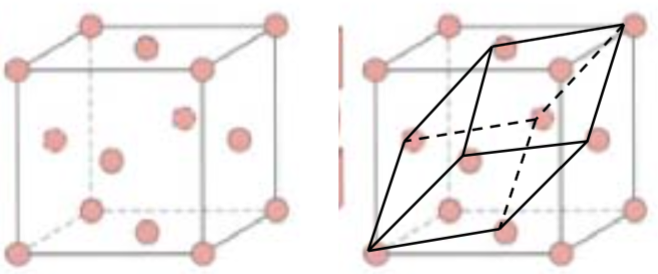
\includegraphics[scale=0.5]{ch4/4}
		\end{wrapfigure}		
		Un exemple est la structure cubique à faces centrées. La maille unitaire primitive la plus simple est de prendre un rhomboèdre (prisme dont les faces sont des losanges identiques) dont les 3 vecteurs primitifs de longueur $a^*$ forment des angles de $60\degres$ entre eux. Cette maille ne contient qu'un seul motif car chaque noeud est partagé entre 8 mailles voisines. Cependant, la symétrie cubique est mieux rendue en prenant une maille unitaire non primitive dont les vecteurs sont perpendiculaires entre eux, de longueur $\sqrt{2}a^*$. Celui-ci contient 4 motifs par maille.
	
\section{Classification des symétries cristallines}
	\subsection{Opérations de symétrie}
		Il y a normalement de nombreuses autres symétries que la translation. Nous allons nous contenter de décrire la symétrie du motif et celle du réseau. On peut démontrer que le nombre d'opération dans l'espace 3D à considérer est limité à 7 : 
		\begin{enumerate}
			\item La translation 
			\item La réflexion par rapport à un plan miroir
			\item La rotation autour d'un axe
			\item L'inversion par rapport à un point de l'espace
			\item L'inversion accompagné d'une rotation
			\item La réflexion par rapport à un plan accompagnée d'une translation le long du plan
			\item La rotation autour d'un axe accompagnée d'une translation le long de cet axe\\
		\end{enumerate}
	
		\begin{wrapfigure}[7]{r}{6cm}
		\vspace{-5mm}
		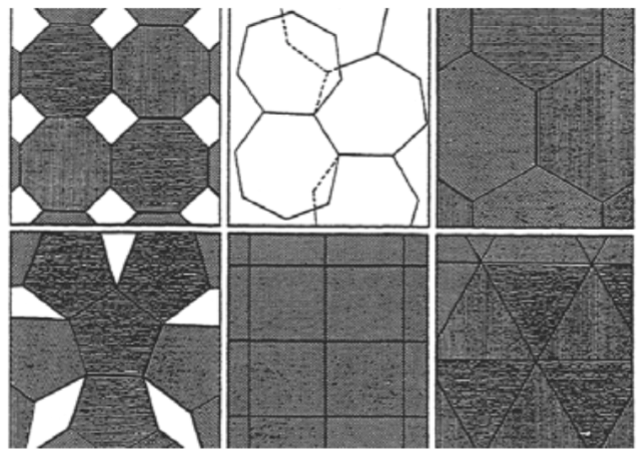
\includegraphics[scale=0.5]{ch4/5}
		\end{wrapfigure}		
		Tout ça compatible avec la translation qui est une caractéristique de base de tout cristal. De ce fait, les seules rotations admissibles sont celles d'angles $2\pi , \pi 2\pi /3 , \pi /2$ et $\pi /3$ (ordre 1,2,3,4 et 6). On peut voir ça sur le schéma ci-contre qui montre qu'il est impossible de remplir un plan en accolant des polygones réguliers à 5,7,8 et plus de côtés.
		
		\newpage
	
	\subsection{Les symétries (sans motifs)}
		\begin{wrapfigure}[12]{l}{11cm}
		\vspace{-5mm}
		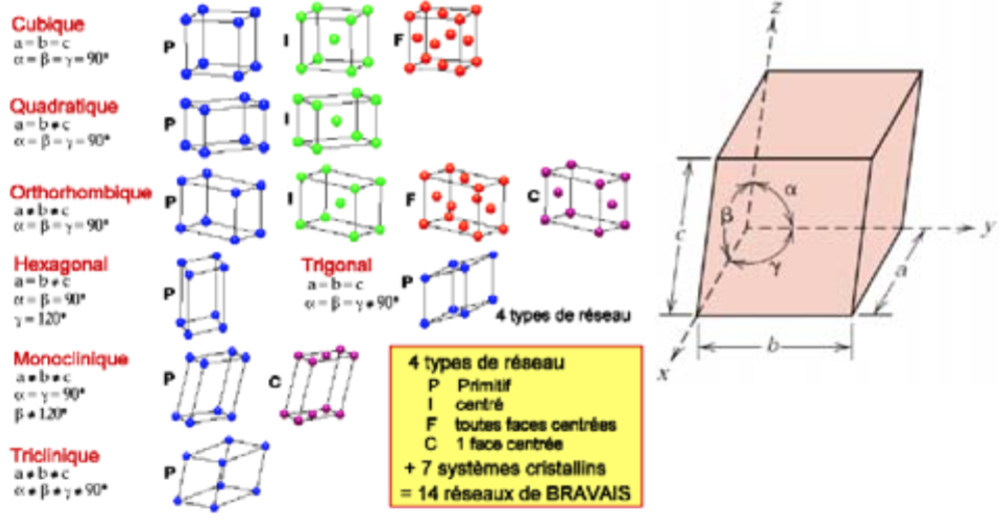
\includegraphics[scale=0.6]{ch4/6}
		\end{wrapfigure}		
		En faisant abstraction des symétries du motifs, le nombre de réseaux différents qu'il est possible de créer est limité à 14 : \textbf{Les 14 réseaux de Bravais}. La représentation en maille unitaire se trouve ci-contre. Seulement la moitié de celles-ci sont unitaires. On peut encore regrouper ces réseaux en 7 catégories plus simples que nous appelons \textbf{systèmes cristallins}. Le degré de symétrie appartenant à ces systèmes augmente avec le nombre de restrictions sur les dimensions relatives des trois vecteurs $a,b$ et $c$ définissant la maille unitaire et sur les angles $\alpha , \beta$ et $\gamma$ que ces vecteurs forment entre eux ($\alpha$ = angle entre $b$ et $c$). 
		
	\subsection{Avec les motifs}
		Le nombre de symétrie que peut présenter le motif d'un cristal est limité à 32 appelés \textbf{32 groupes de symétrie}. Le réseau qui accueille le motif doit présenter une symétrie au moins égal à celle du motif. En effet, une opération de symétrie effectué sur un cristal doit laisser inchangés à la fois le motif et le réseau. On peut alors associer à chaque groupe ponctuel le réseau de Bravais possédant la symétrie minimale pour accueillir ce groupe. \\ Ce n'est pas tout, l'association du motif et du réseau augmente encore le nombre de symétries possibles. On a un total de 230 types de structures possibles que l'on dénomme \textbf{230 groupes de symétries spaciaux}. 
		
	
\section{Directions cristallines et indices de Miller}
	\subsection{Notation des directions}
		\begin{wrapfigure}[10]{r}{7cm}
		\vspace{-10mm}
		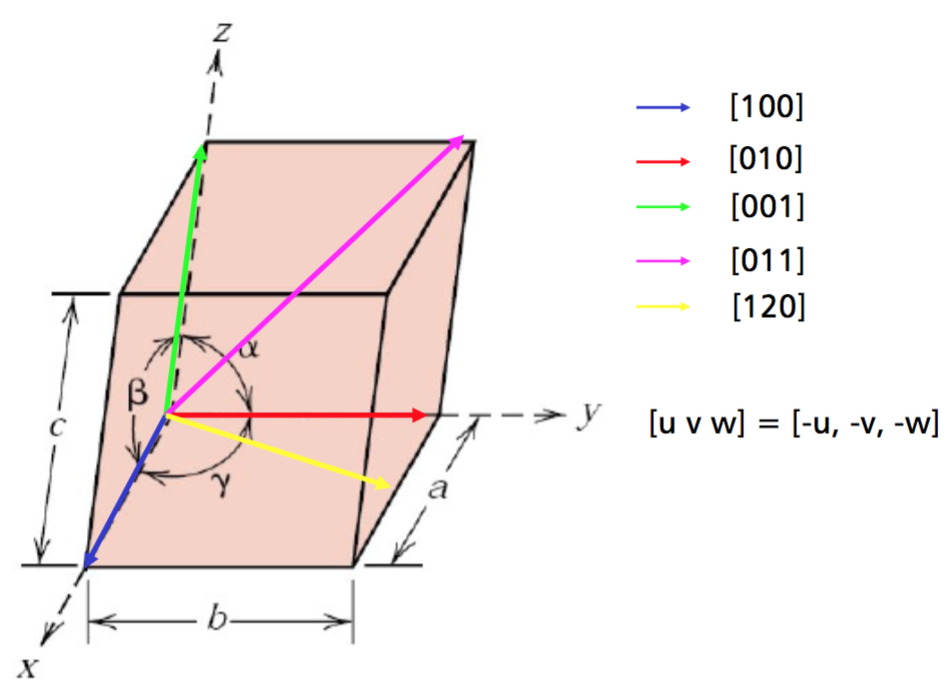
\includegraphics[scale=0.4]{ch4/7}
		\end{wrapfigure}	
		Le nom donné à une direction ou à un plan dépend de la maille unitaire choisie. Considérons la maille définie ci-contre par les vecteurs $a,b$ et $c$. Ceux-ci forment un système dextrogyre dont l'origine définit celle du réseau. Un point quelconque de la maille sera désigné par les trois coordonnées de ce point dans ce système (ex : atome au centre de la face inférieur $\rightarrow \frac{1}{2},\frac{1}{2},0$; sans parenthèses). \\
		Pour un noeud quelconque d'un réseau définit par
		\begin{equation}
			r = u_1 a + v_1b+w_1c
		\end{equation}
		tous les noeuds $u_i,v_i$ et $w_i$ tels que $\frac{u_i}{u_1} = \frac{v_i}{v_1} = \frac{w_i}{w_1}$ appartiennent à une même rangée passant par l'origine. On note la direction d'une rangée par le symbole $[u,v,w]$ et on surmonte les nombres négatifs d'un trait horizontal (ex : $[u,-v,-w] \rightarrow [u;\bar{v},\bar{w}]$). Pour tous les systèmes autres que le système monoclinique, la symétrie du réseau implique que plusieurs directions sont équivalentes, c'est à dire qu'elles ont le même environnement d'atomes et que les propriétés seront donc les même dans ces directions. Par exemple, pour un cube, les directions $[1,0,0],[0,1,0],[0,0,1],[-1,0,0],[0,-1,0],[0,0,-1]$. On note ça en abrégé $<1\, 0 \, 0>$. Si la direction envisagée ne passe pas par l'origine, il suffit de translater l'origine. 
		
	\subsection{Notation de plans : indice de Miller}
		\begin{center}
		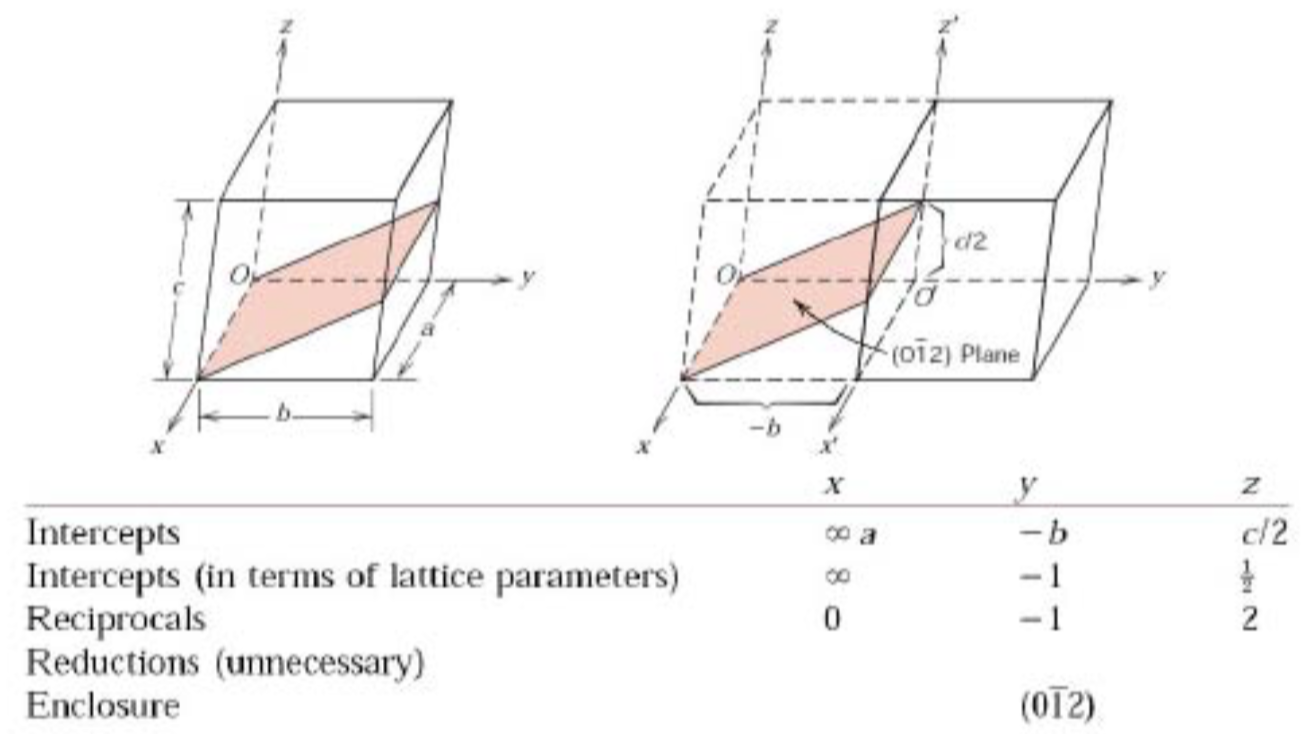
\includegraphics[scale=0.45]{ch4/8}
		\end{center}	
		On désigne un plan grâce à trois indices, appelés indice de Miller. Ceux-ci sont les inverses des intersections du plan avec les trois axes du cristal. La recette : 
		\begin{enumerate}
			\item Si le plan passe par l'origine, translater l'origine.
			\item Déterminer les coordonnées des intersections du plan avec les axes en fonctions des vecteurs a, b, c qui définissent la maille unitaire. 
			\item Prendre l'inverse de chacune de ces intersections. Si le plan ne coupe pas un axe, son intersection est à l'infini et l'inverse fait 0.
			\item Réduire les trois fonctions ainsi obtenue au plus petit commun dénominateur.
			\item Les trois numérateurs h, k, l, sont les trois indices de Miller du plan.
			\item On le note $(hkl)$
		\end{enumerate}
		Comme pour les directions cristallines, la symétrie des systèmes cristallins entraîne l'équivalence de familles de plan d'indices de Miller différents. On désigne l'ensemble des familles par le symbole ${h \, k \, l}$. 